\section{Sprint Closure}
% What did we do?
% We solved our issues, made a usability test, code review with another group, 
The issues mentioned in the sprint backlog have been solved but new issues have also been discovered through the usability test as mentioned in \secref{sec:usability-test}.
Replacement of pictograms in the database was not implemented in the sprint, but is recommended to consider for future groups that are further developing \textit{Piktotegner}.

We also refactored the code such that it is easier to understand for future developers.
The refactored code was also shown to another development group as part of a code review and gave us feedback.
The feedback was taken into consideration and changes were performed when they were deemed reasonable.
The resulting code should now be easier for the next development group to expand upon if further development of this application is performed.

% New issues brought up on sprint end
After the presentation of the application during the sprint end meeting, new issues were mentioned which are added to the product backlog.
An example of an issue was that the audience were slightly confused of what the preview button was actually doing, so a rethinking of this button should be done.

The final UI of \textit{Piktotegner} can be seen in \figref{fig:main_ui}.

\begin{figure}[h]
	\centering
	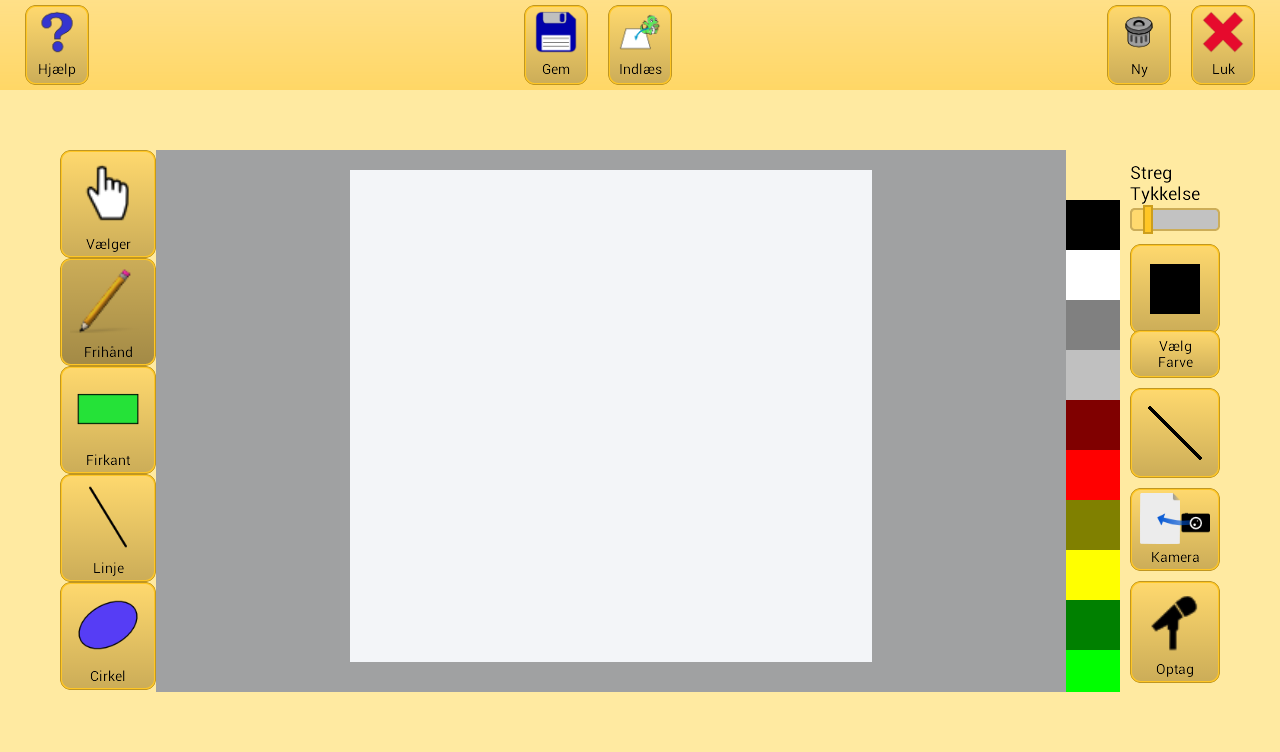
\includegraphics[width=\textwidth]{media/sprint4/final-main-ui}
	\caption{The final UI of \textit{Piktotegner}.}
	\label{fig:main_ui}
\end{figure}


This concludes the development phase of the project, all remaining issues are written in the product backlog for easy reference for future developers, see \appref{app:further-deflopment}.